\documentclass[xcolor={dvipsnames}]{beamer}
%\usepackage[margin=1.0in]{geometry}

\usepackage[utf8]{inputenc}
\usepackage[english]{babel}
\usepackage[T1]{fontenc}
\usepackage{lmodern}

%----------------------------------------------------------------------------------------
%	MATH PACKAGES
%----------------------------------------------------------------------------------------

% Banish \phi from this realm
\renewcommand{\phi}{\varphi}

\usepackage{amsmath, amssymb, mathrsfs}
\usepackage{mathtools}

%----------------------------------------------------------------------------------------
%	DEFINING NEW FUNCTIONS
%----------------------------------------------------------------------------------------

% --------- MATH MODE ---------
% Equation numbering per section
\numberwithin{equation}{section}

% \cdot instead of asterisk (*) symbol
\mathcode`\*="8000
{\catcode`\*\active\gdef*{\cdot}}

% --------- OTHER ---------

\usepackage[dvipsnames]{xcolor}

% tikz
%\usepackage{tikz}

% Captions
\usepackage[font=scriptsize]{caption}

% Quotes
\usepackage[autostyle=false]{csquotes}
\newcommand{\q}[1]{„#1''} % Redefine quotations

\usetheme{Madrid}
\usecolortheme{default}
\setbeamertemplate{caption}[numbered]

\newif\ifplacelogo
\placelogotrue
%----------------------------------------------------------------------------------------
%	TITLE PAGE
%----------------------------------------------------------------------------------------
\title[Geant4]
{Simulation of the NEBULA detector using Geant4}

\subtitle{Midterm presentation}

\author[Balázs Pál]
{Balázs Pál}

\institute[ELTE]
{
  Supervisor : Ákos Horváth, PhD \newline
  Eötvös Loránd University
}

\date[ELTE 2021]
{Scientific Modelling Computer Lab, March 24, 2021}

\logo{\ifplacelogo
\includegraphics[height=1.5cm]{./images/elte-logo.jpg}\fi}

\begin{document}

\frame{\titlepage}
%----------------------------------------------------------------------------------------
%	SLIDE 1.
%----------------------------------------------------------------------------------------
\begin{frame}
\frametitle{Simulation of the NEBULA detector}

\begin{block}{Initial considerations}
	\begin{itemize}
		\item Installing smsimulator, which uses libraries from ROOT and ANAROOT and headers and binaries from Geant4
		\item This software could be used to simulate the NEBULA detector with very high accuracy
		\item Installing and configuring it seems to be a nightmare currently
	\end{itemize}
\end{block}

\pause

\begin{alertblock}{Changed roadmap}
	\begin{itemize}
		\item Temporarily abort the idea of using smsimulator
		\item Implementing a simplified version of the NEBULA  detector
		\item It should be still able to give good approximations
	\end{itemize}
\end{alertblock}

\end{frame}
%----------------------------------------------------------------------------------------
%	SLIDE 2.
%----------------------------------------------------------------------------------------
\begin{frame}
\frametitle{NEBULA detector}
\framesubtitle{\textbf{NE}utron Detection System for \textbf{B}reakup of \textbf{U}nstable Nuclei with \textbf{L}arge \textbf{A}cceptance}

\begin{block}{Detector geometry}
	\begin{itemize}
		\item Designed to detect fast neutrons at $100$-$300$ MeV
		\item Consist of $4$ bigger blocks
		\item Each block consist of $60$, BC-$408$ plastic scintillator rods
	\end{itemize}
\end{block}

\begin{figure}
	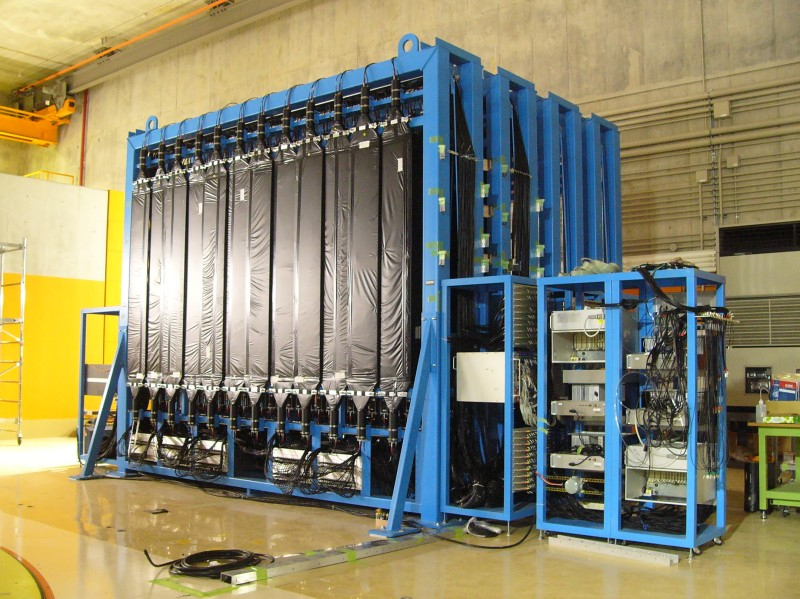
\includegraphics[width=0.5\textwidth]{images/nebula_detector.jpg}
\end{figure}

\end{frame}
%----------------------------------------------------------------------------------------
%	SLIDE 3.
%----------------------------------------------------------------------------------------
\begin{frame}
\frametitle{Simulations in Geant4}
\framesubtitle{Very short outline}

\begin{block}{Usual components}
	\begin{itemize}
		\item Detector construction
		\item Particle generation
		\item Data I/O
		\item Core loop
	\end{itemize}
\end{block}

\end{frame}
%----------------------------------------------------------------------------------------
%	SLIDE 4.
%----------------------------------------------------------------------------------------
\begin{frame}
\frametitle{NEBULA detector in the simulation}

\begin{exampleblock}{Structure and composition}
	\begin{itemize}
		\item $2 \times 10$ plastic scintillator rods in two layers
		\item Dimensions of rods are $12\text{cm} \times 12\text{cm} \times 180\text{cm}$
		\item Filled with the BC-$408$ pastic scintillator material ($52.45\%$ H and $47.55\%$ C)
	\end{itemize}
\end{exampleblock}

\begin{figure}
	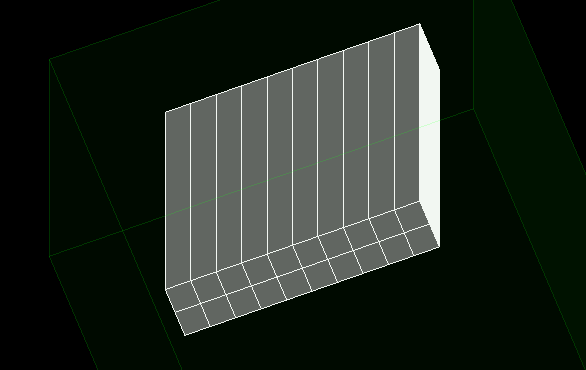
\includegraphics[width=0.5\textwidth]{images/nebula.png}
\end{figure}


\end{frame}
%----------------------------------------------------------------------------------------
%	SLIDE 5./1.
%----------------------------------------------------------------------------------------
\begin{frame}
\frametitle{Processes during a simulation}

\begin{block}{}
	\begin{itemize}
		\item With different \texttt{physics list} we'll obtain different results (again)
		\item We can study the energy deposit and occurrence of physical processes individually
	\end{itemize}
\end{block}

\begin{figure}
	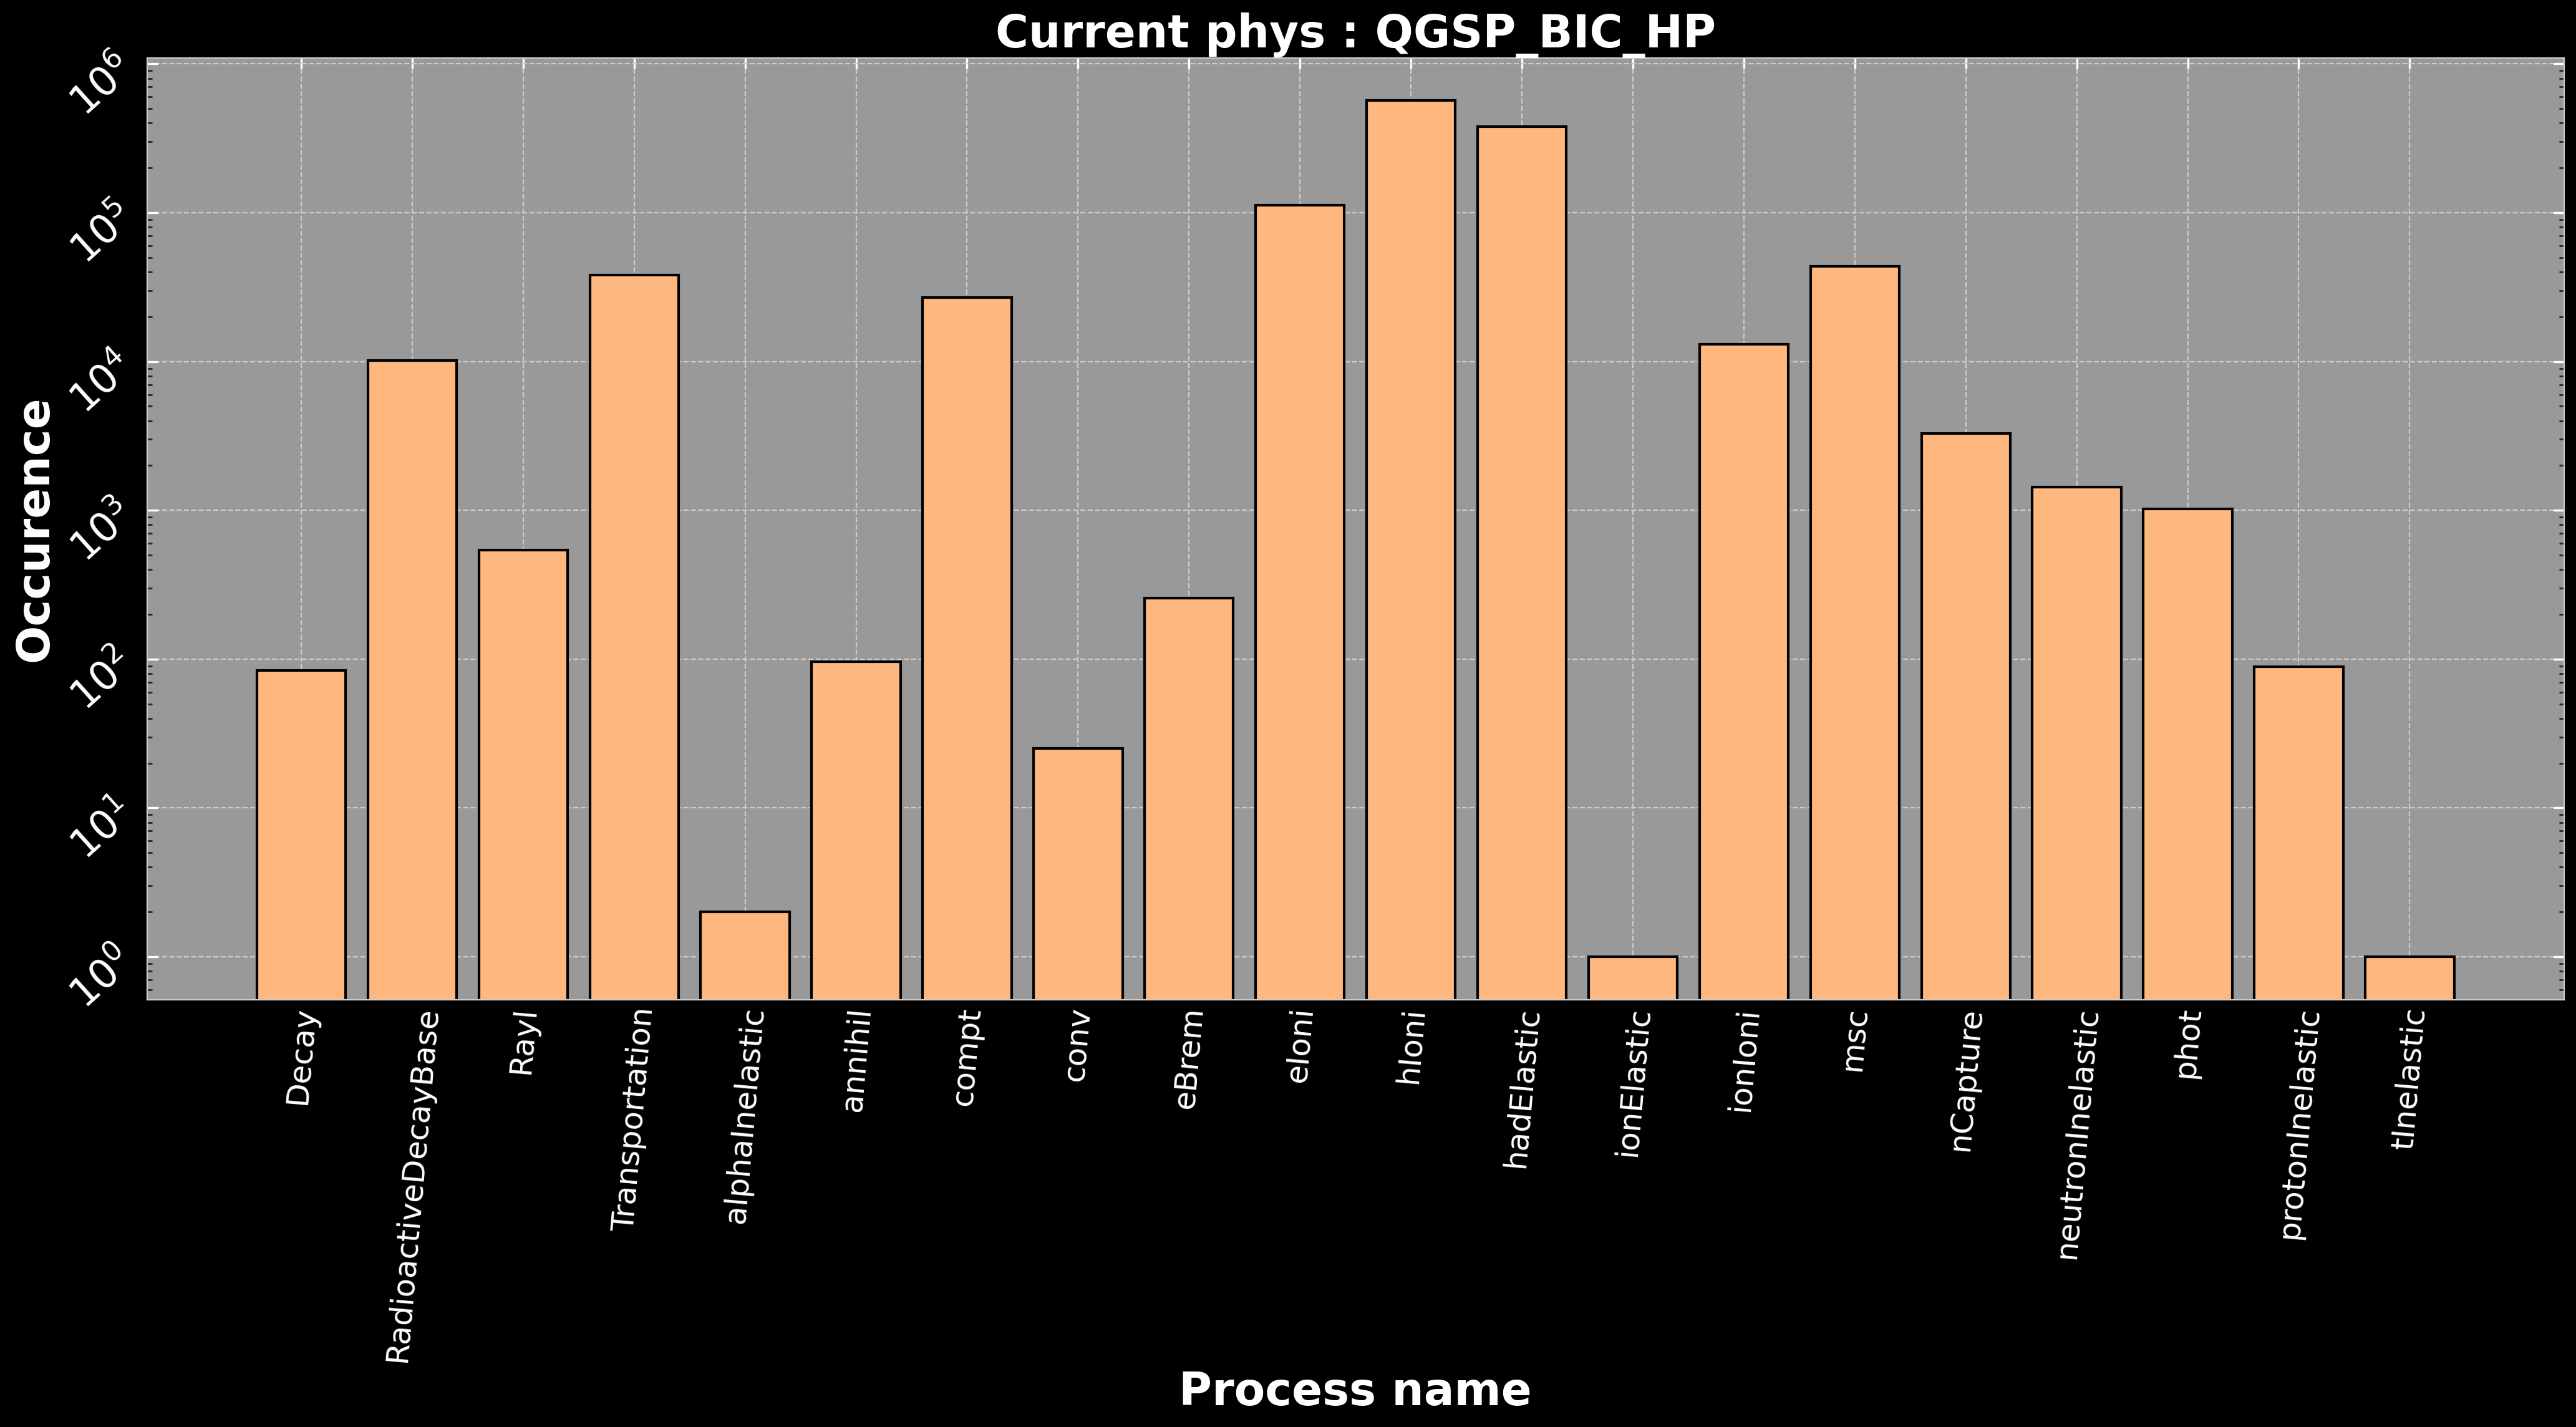
\includegraphics[width=0.8\textwidth]{images/process_dist_E100_phQGSP_BIC_HP.png}
\end{figure}

\end{frame}
%----------------------------------------------------------------------------------------
%	SLIDE 5./2.
%----------------------------------------------------------------------------------------
\begin{frame}
\frametitle{Processes during a simulation}

\begin{block}{}
	\begin{itemize}
		\item With different \texttt{physics list} we'll obtain different results (again)
		\item We can study the energy deposit and occurrence of physical processes individually
	\end{itemize}
\end{block}

\begin{figure}
	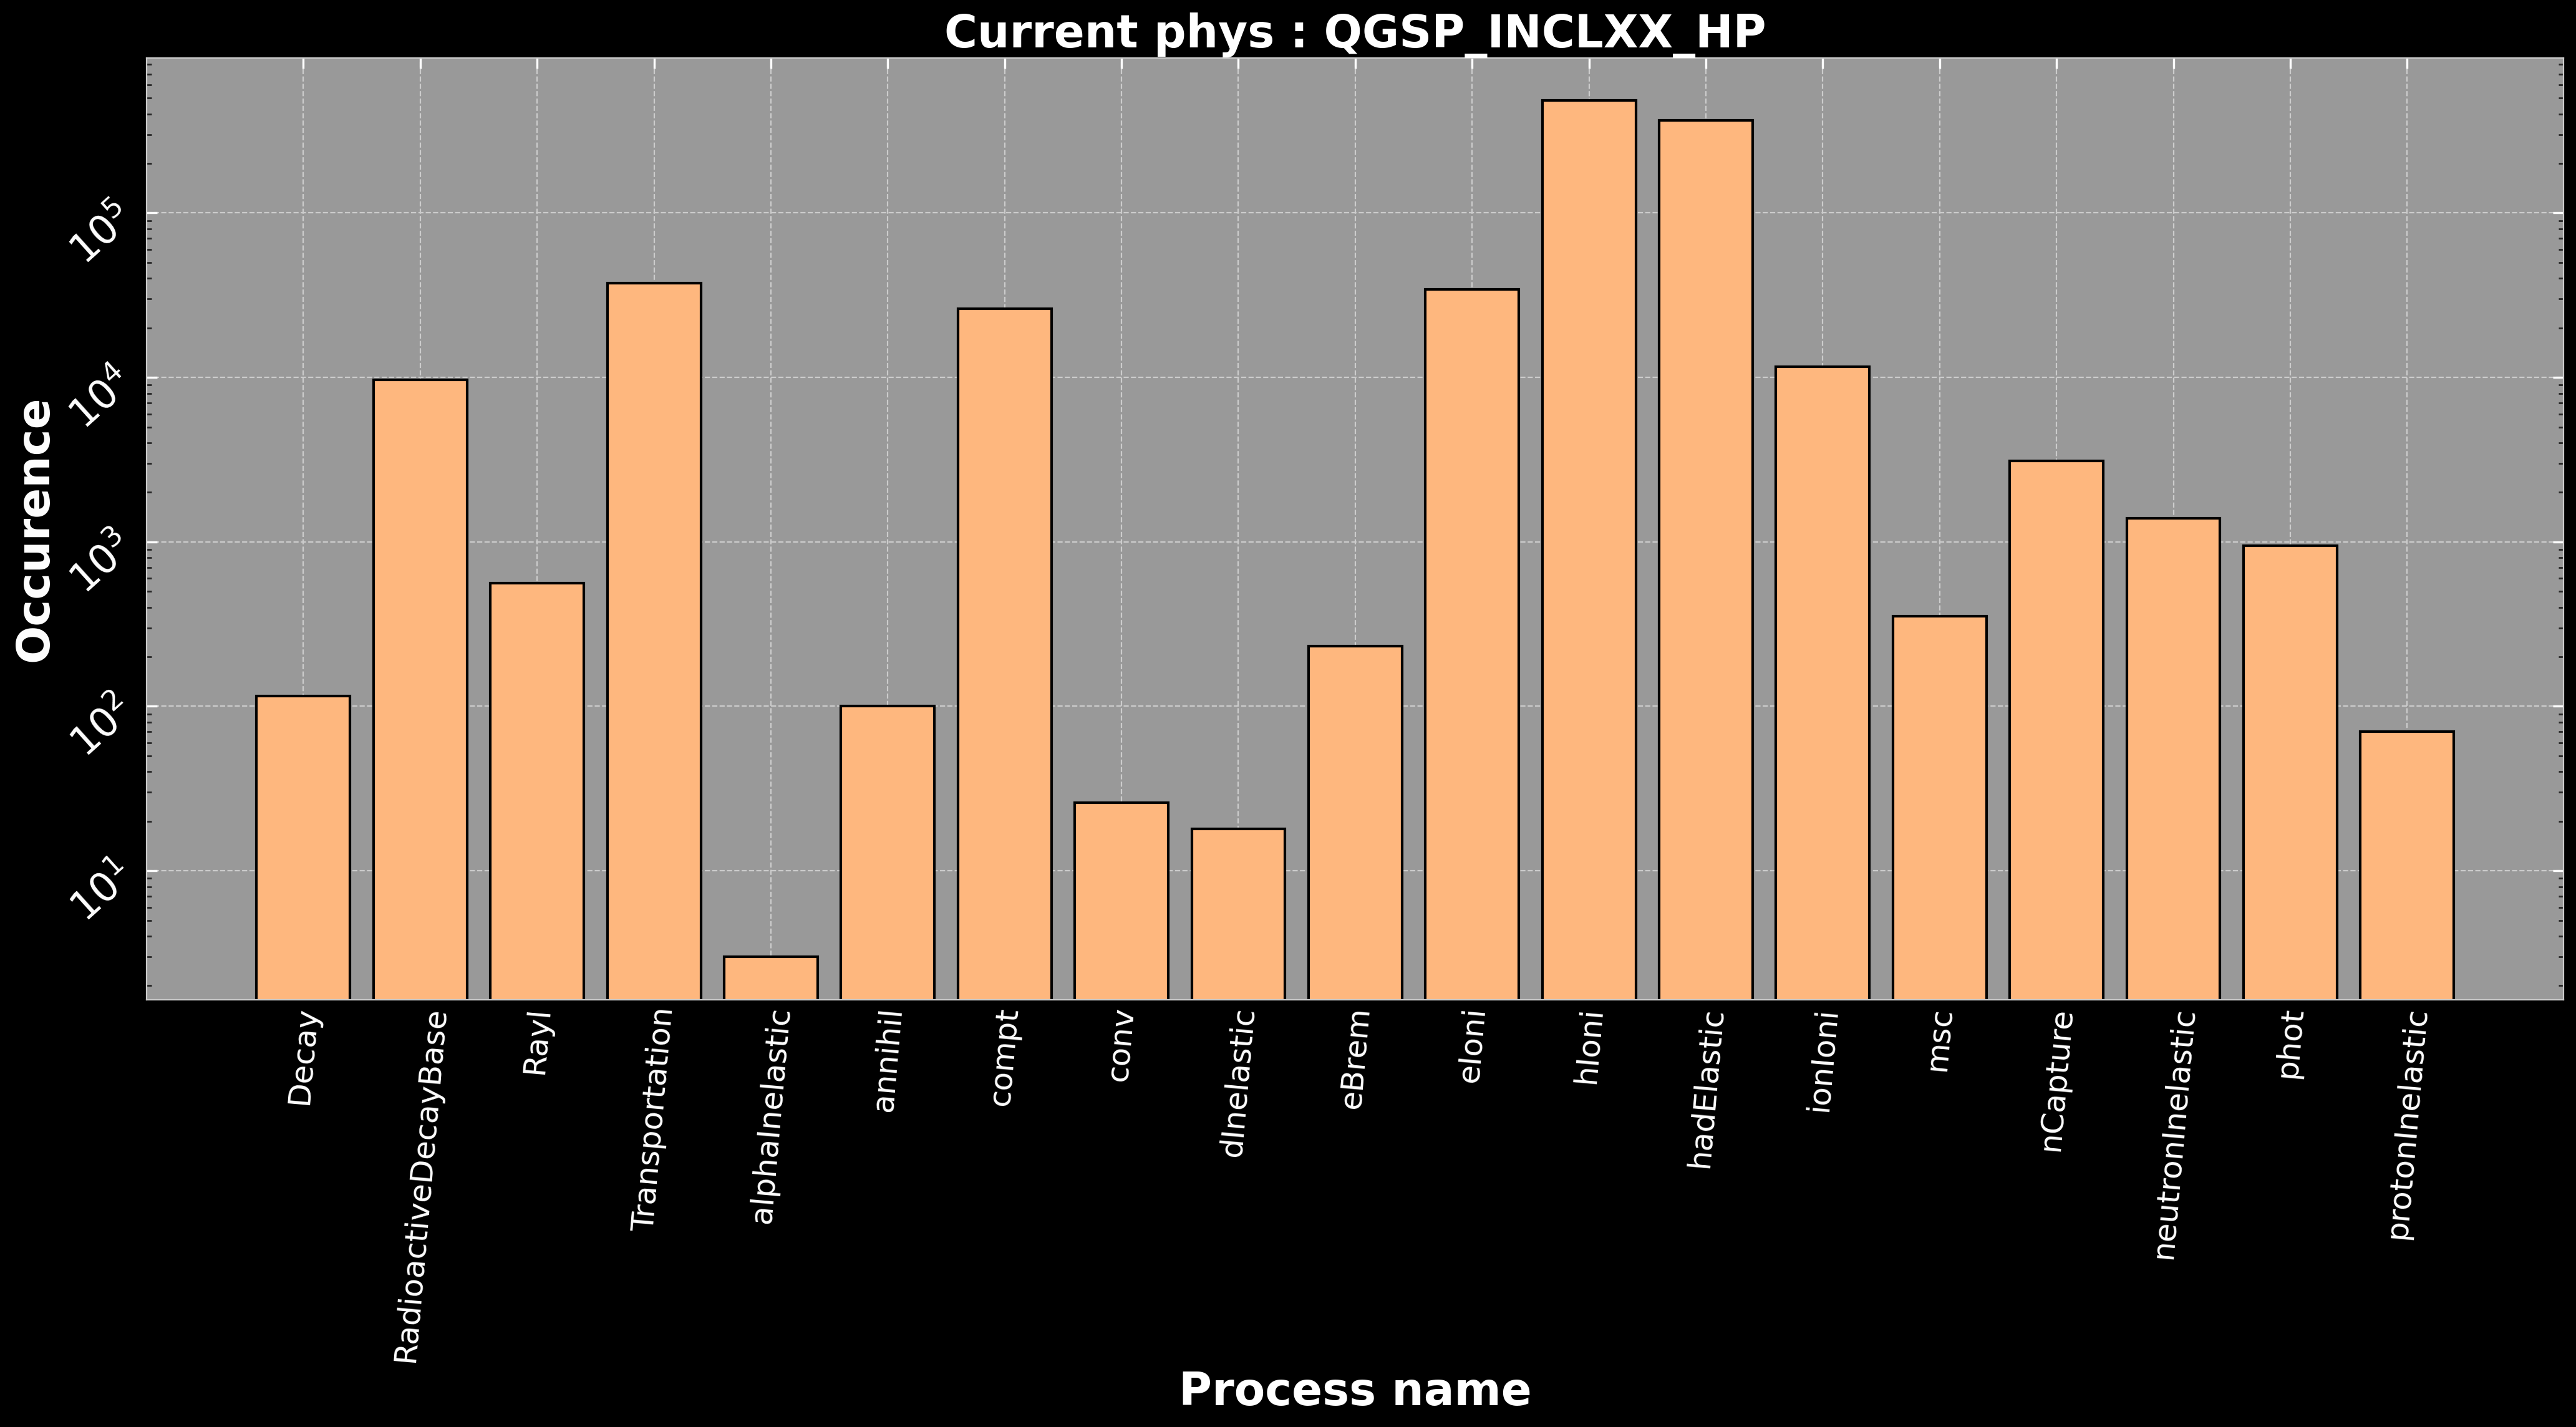
\includegraphics[width=0.8\textwidth]{images/process_dist_E100_phQGSP_INCLXX_HP.png}
\end{figure}

\end{frame}
%----------------------------------------------------------------------------------------
%	SLIDE 5./3.
%----------------------------------------------------------------------------------------
\begin{frame}
\frametitle{Processes during a simulation}

\begin{block}{}
	\begin{itemize}
		\item With different \texttt{physics list} we'll obtain different results (again)
		\item We can study the energy deposit and occurrence of physical processes individually
	\end{itemize}
\end{block}

\begin{figure}
	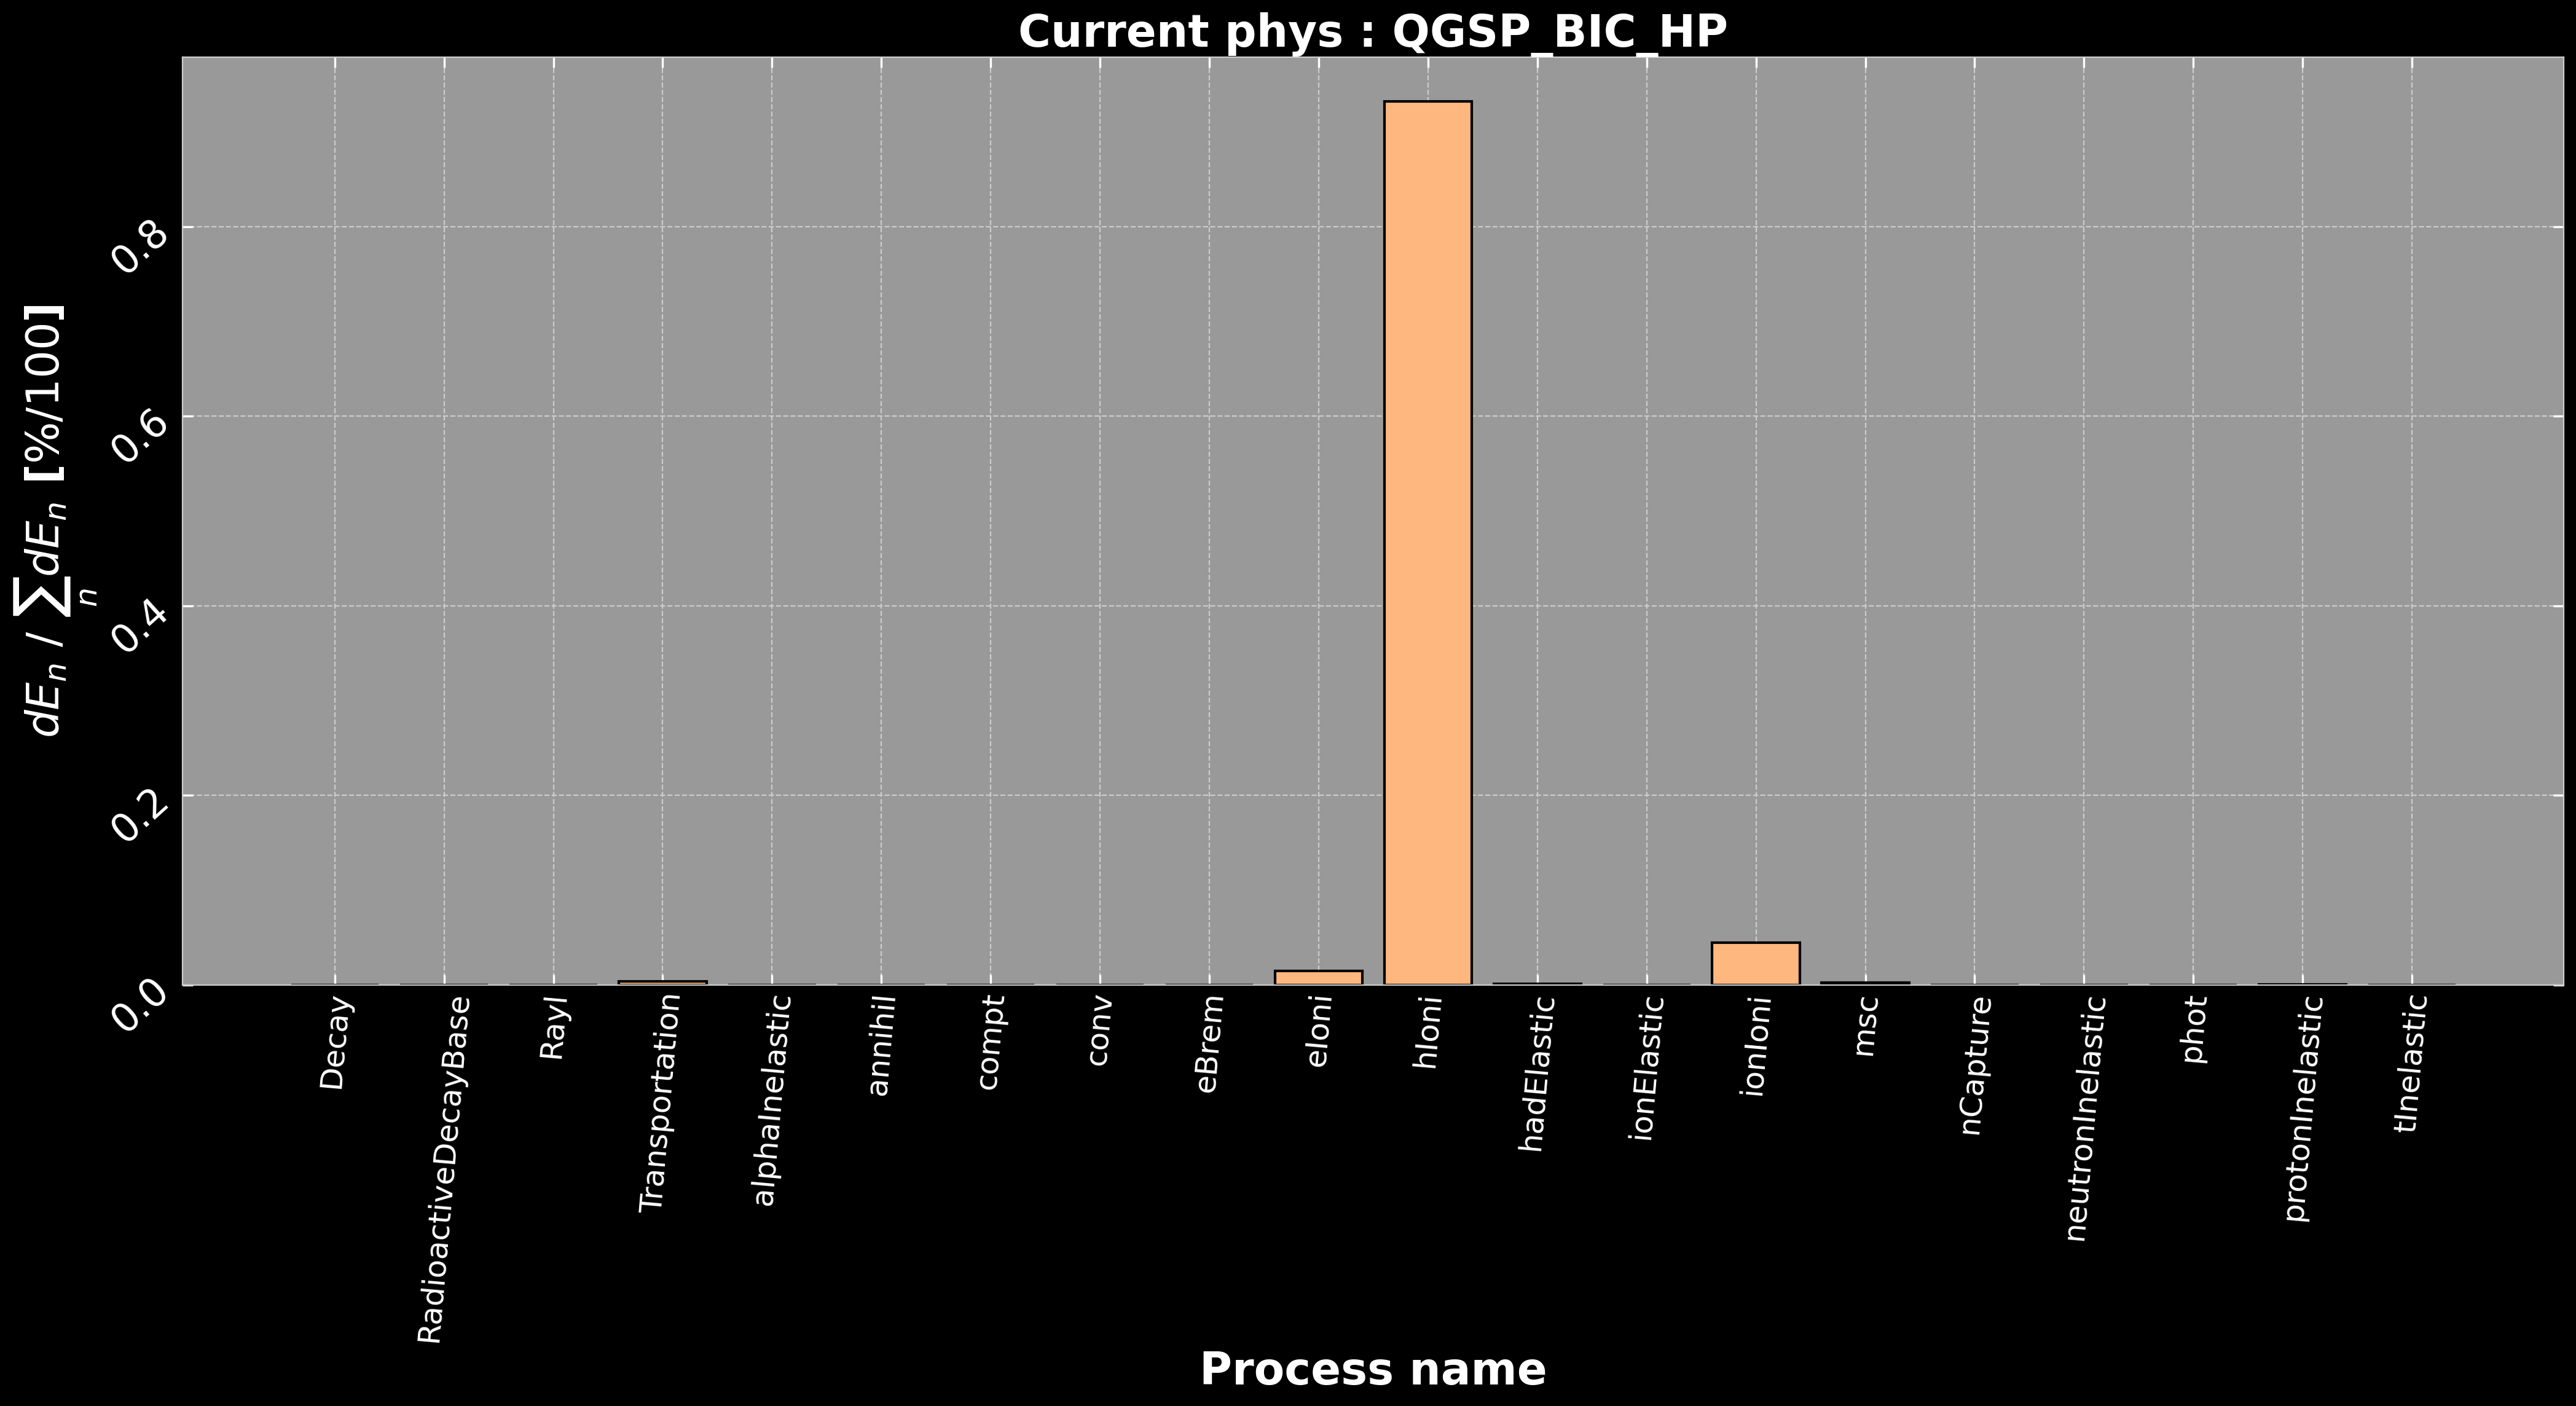
\includegraphics[width=0.8\textwidth]{images/process_dist_weighted_E100_phQGSP_BIC_HP.png}
\end{figure}

\end{frame}
%----------------------------------------------------------------------------------------
%	SLIDE 5./4.
%----------------------------------------------------------------------------------------
\begin{frame}
\frametitle{Processes during a simulation}

\begin{block}{}
	\begin{itemize}
		\item With different \texttt{physics list} we'll obtain different results (again)
		\item We can study the energy deposit and occurrence of physical processes individually
	\end{itemize}
\end{block}

\begin{figure}
	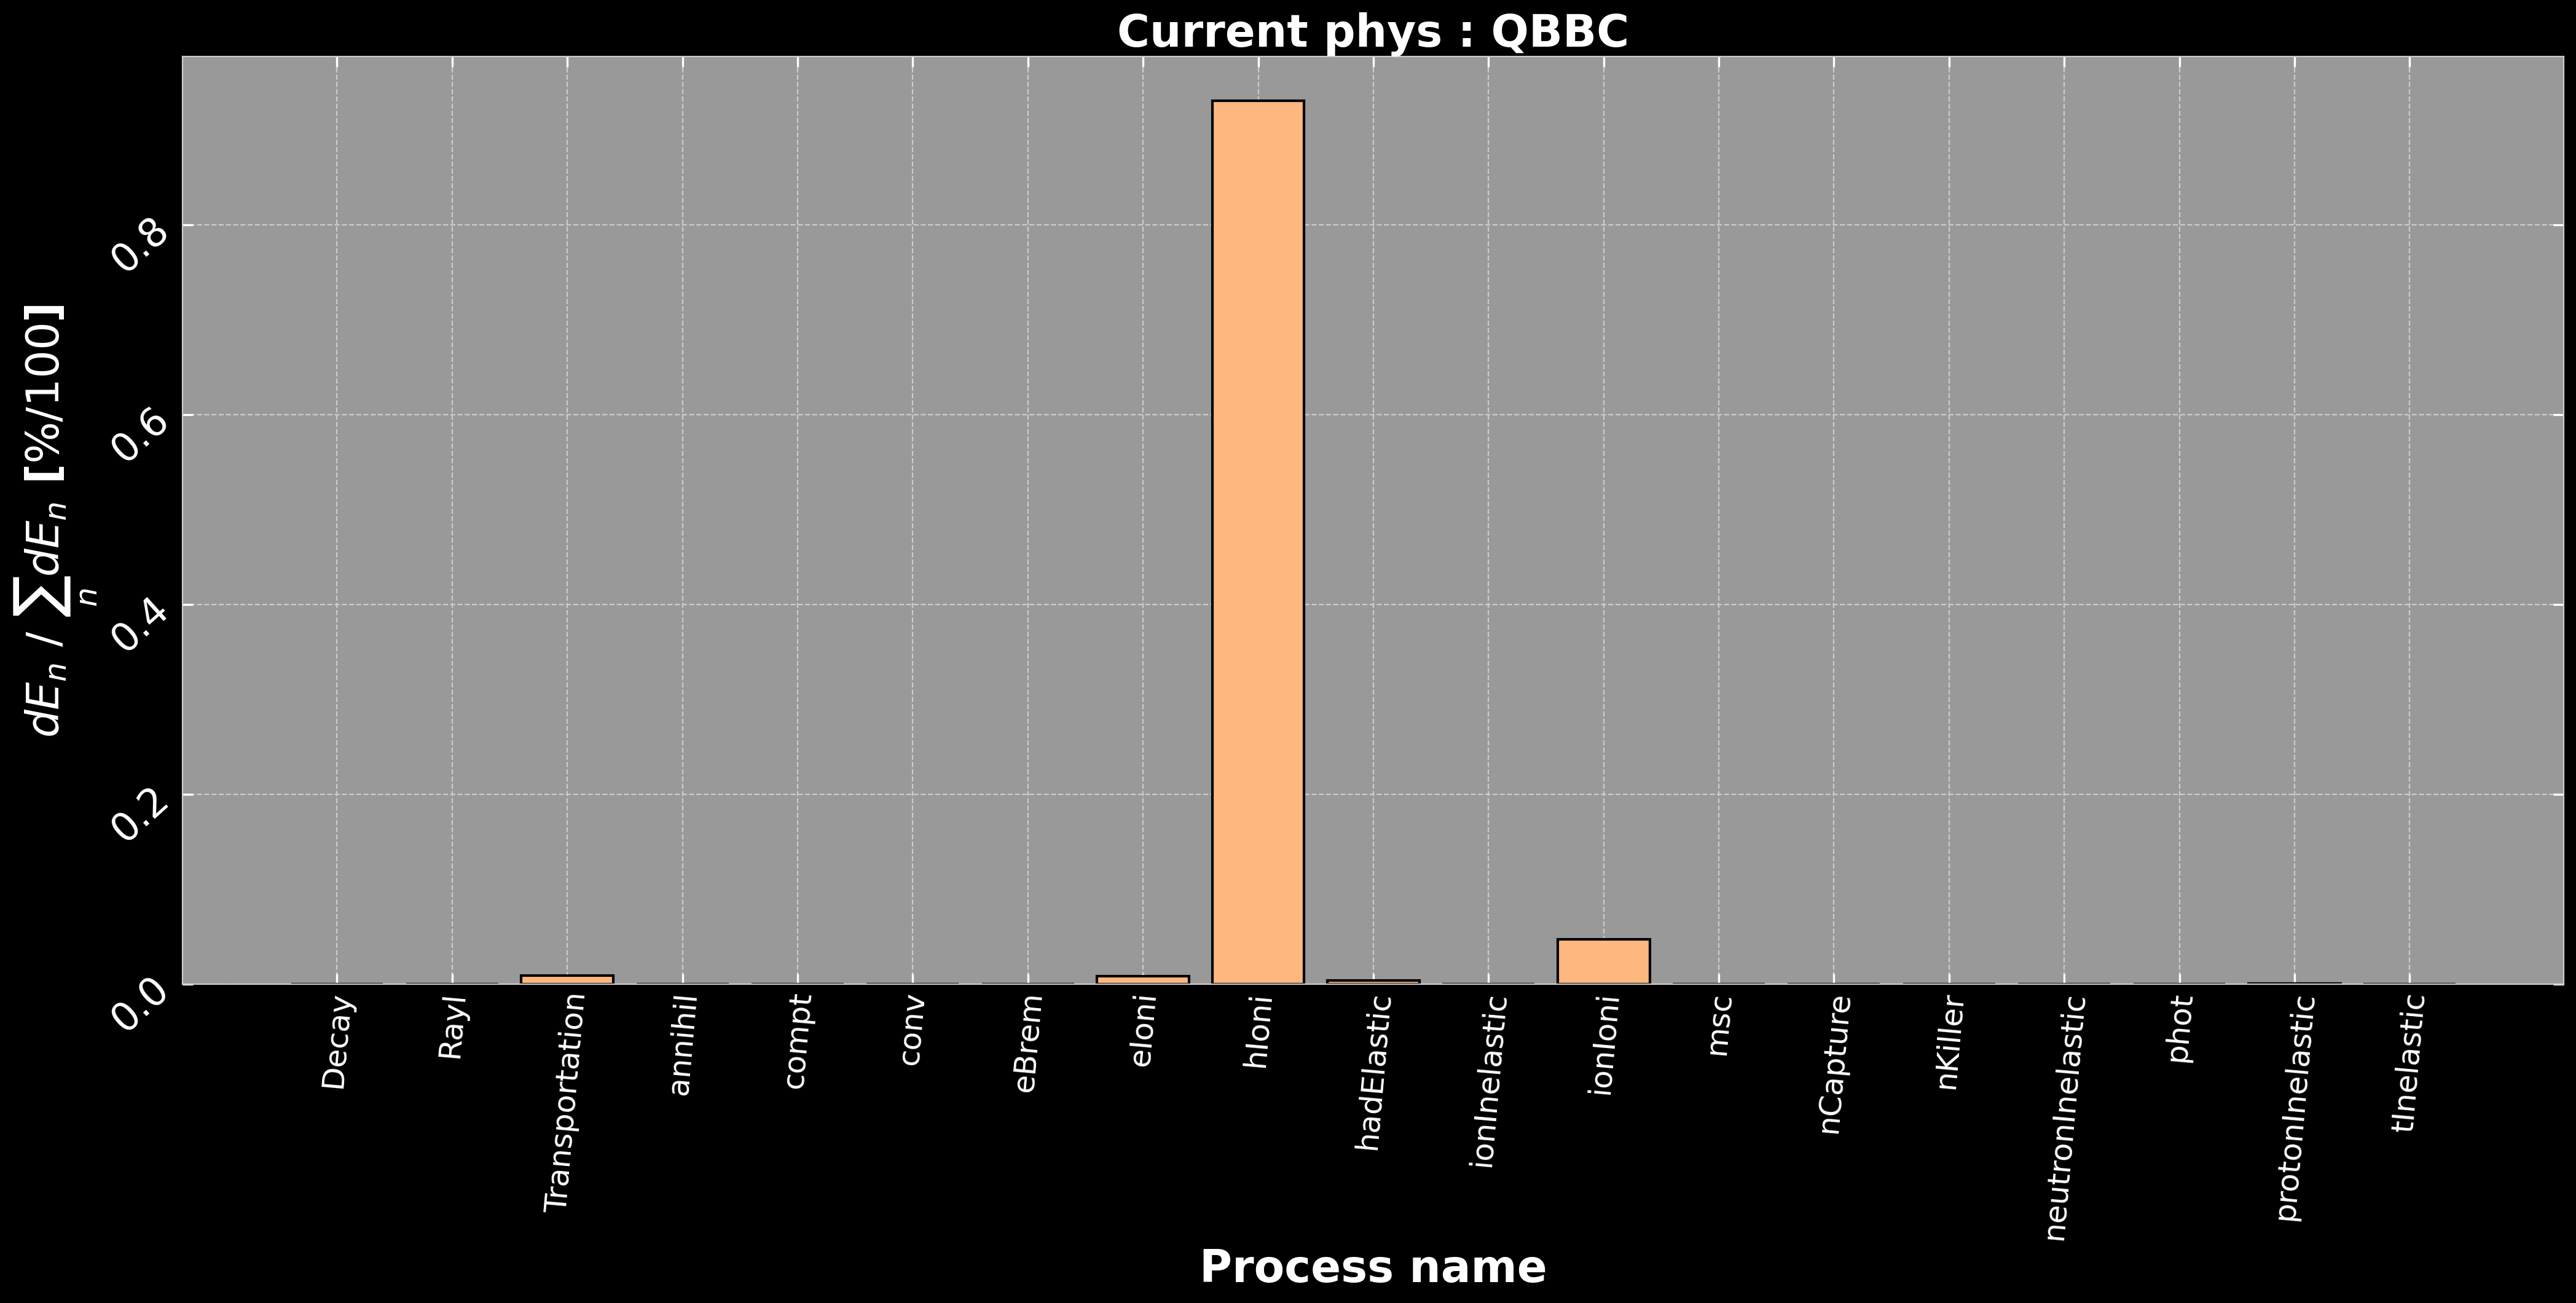
\includegraphics[width=0.8\textwidth]{images/process_dist_weighted_E100_phQBBC.png}
\end{figure}

\end{frame}
%----------------------------------------------------------------------------------------
%	SLIDE 6.
%----------------------------------------------------------------------------------------
\begin{frame}
\frametitle{Particles during a simulation}

\begin{figure}
	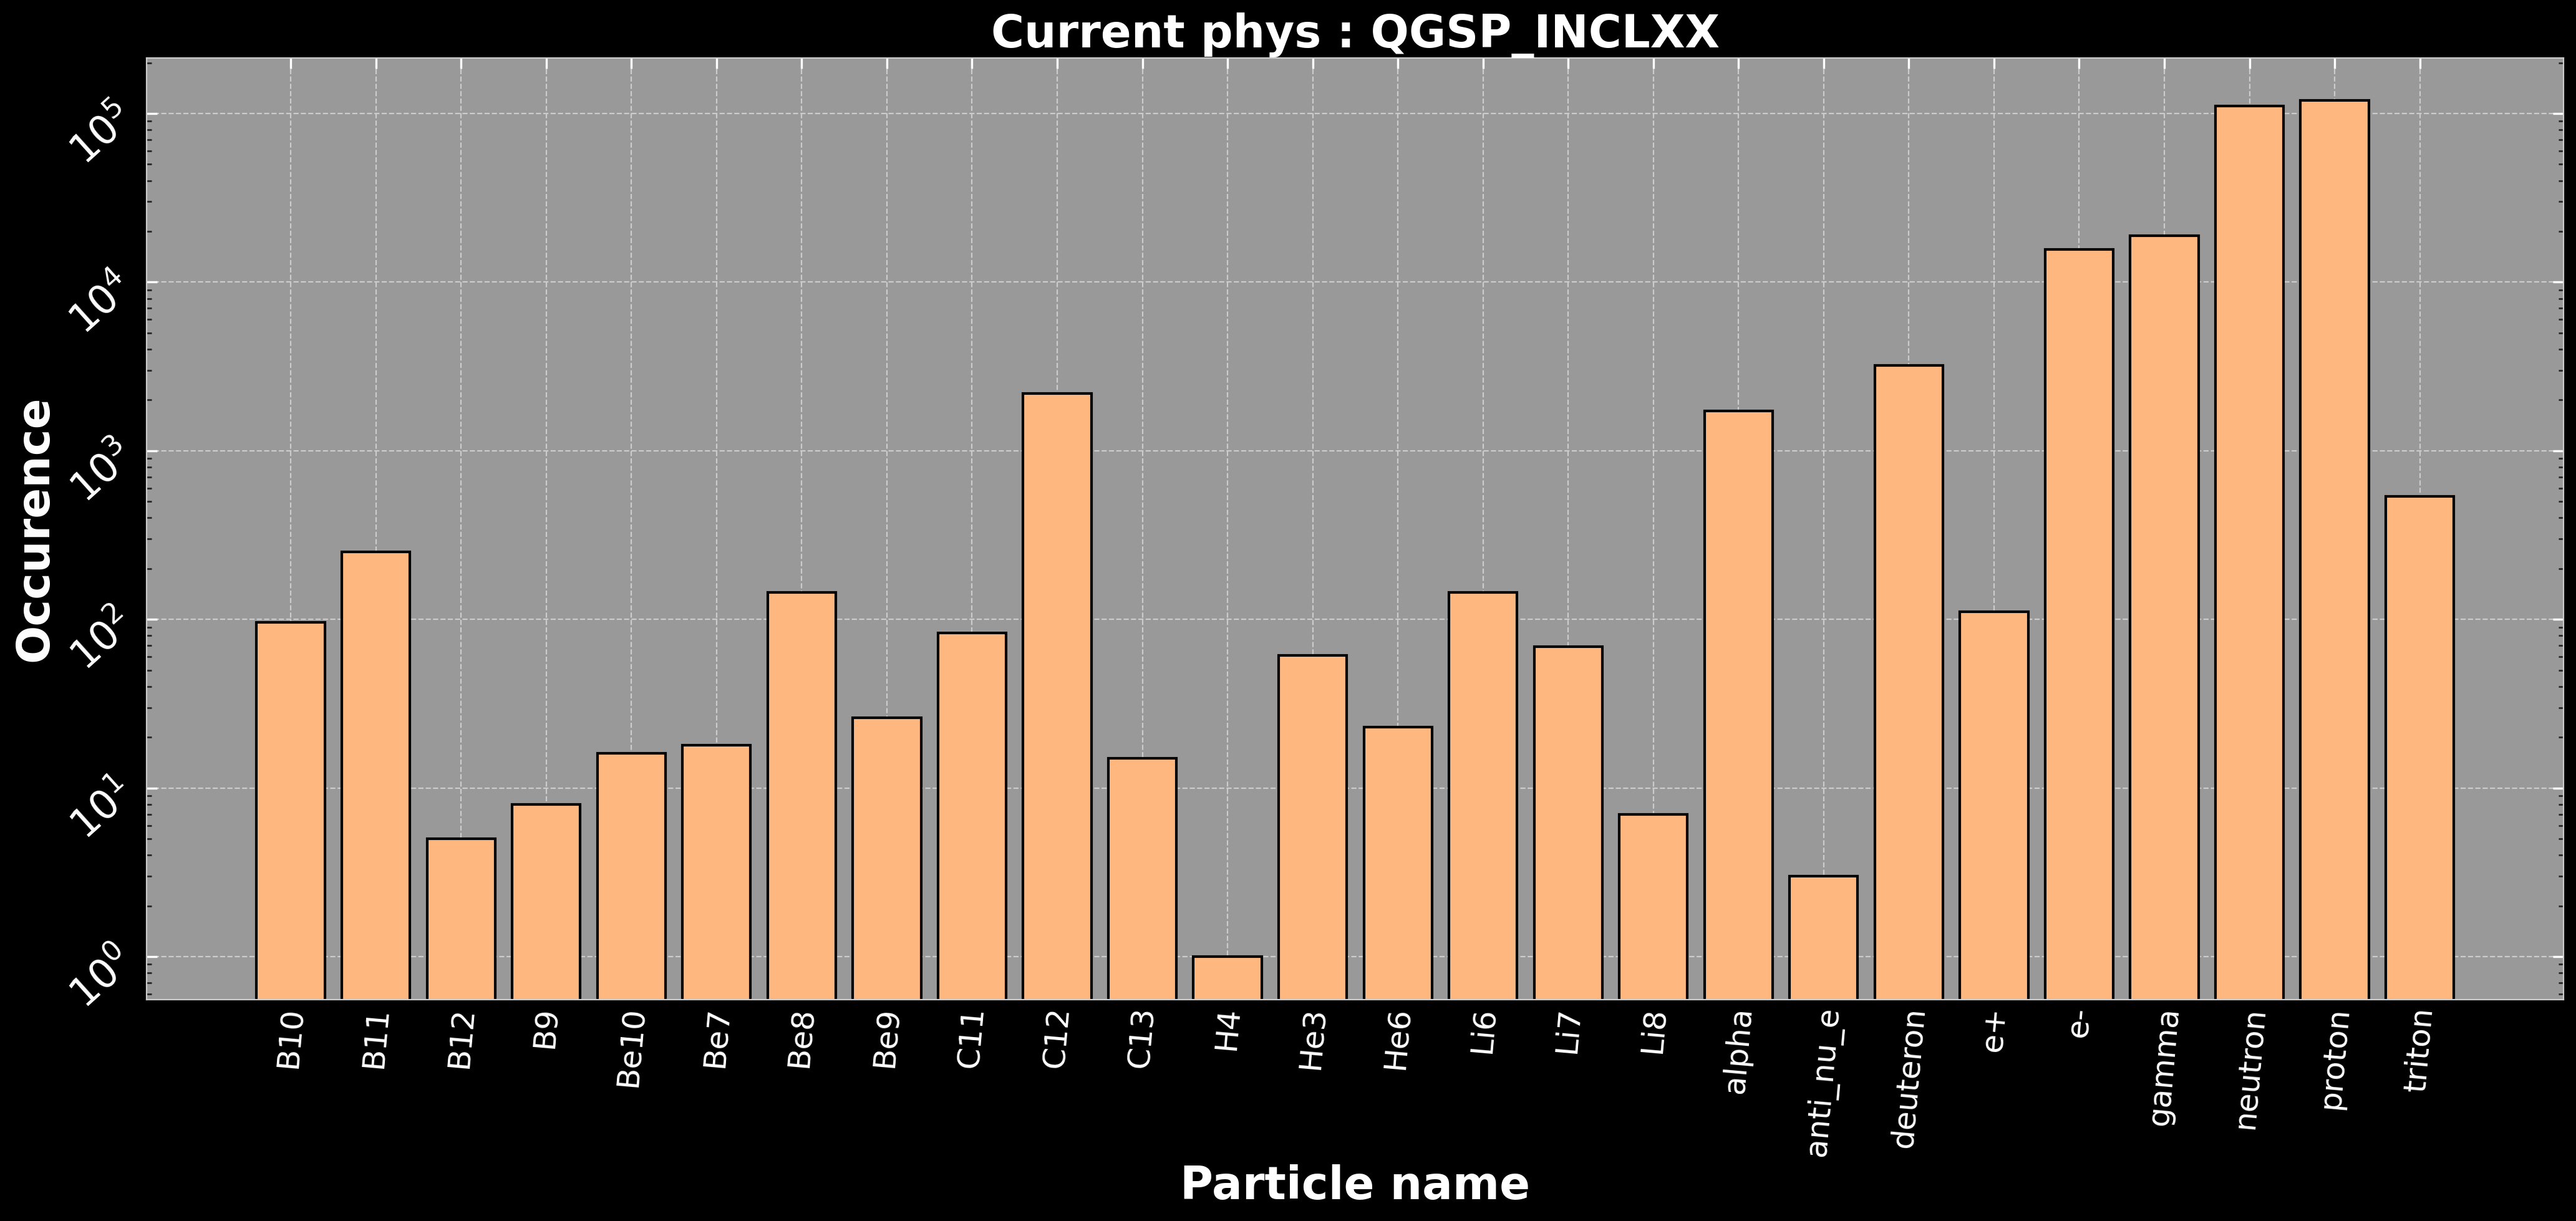
\includegraphics[width=1.0\textwidth]{images/particle_dist_E100_phQGSP_INCLXX.png}
\end{figure}

\end{frame}

\end{document}